\documentclass[12pt,letterpaper]{report}

% -----------------------------------------------------------------------------
% APA 7-style layout based on the supplied Word template
% -----------------------------------------------------------------------------
\usepackage[letterpaper,margin=1in,headheight=15pt,headsep=0.25in]{geometry}
\usepackage[T1]{fontenc}
\usepackage[utf8]{inputenc}
\usepackage{newtxtext,newtxmath} % Times-like text and mathematics
\usepackage{setspace}
\usepackage{indentfirst}
\usepackage{titlesec}
\usepackage{fancyhdr}
\usepackage{csquotes}
\usepackage[hidelinks]{hyperref}
\usepackage{graphicx}
\usepackage{float}
\usepackage{booktabs}
\usepackage{caption}
\usepackage{enumitem}
\usepackage[style=apa,backend=biber,sortcites=true,sorting=nyt]{biblatex}
\DeclareLanguageMapping{english}{english-apa}
\addbibresource{references.bib}

% -----------------------------------------------------------------------------
% Editable metadata
% -----------------------------------------------------------------------------
\newcommand{\ThesisTitle}{AI Programming Foundations Capstone Project: Analyzing Airbnb Listings in New York City}
\newcommand{\AuthorName}{Marius Jochheim}
\newcommand{\Institution}{Udacity}
\newcommand{\CourseName}{AI Programming with Python Nanodegree}
\newcommand{\SupervisorName}{}
\newcommand{\SubmissionDate}{\today}

% -----------------------------------------------------------------------------
% Global typography and paragraph layout
% -----------------------------------------------------------------------------
\doublespacing
\setlength{\parindent}{0.5in}
\setlength{\parskip}{0pt}
\raggedbottom
\setlist{nosep}

% Page number at the upper-right, including the title page.
\pagestyle{fancy}
\fancyhf{}
\fancyhead[R]{\thepage}
\renewcommand{\headrulewidth}{0pt}
\fancypagestyle{plain}{%
  \fancyhf{}
  \fancyhead[R]{\thepage}
  \renewcommand{\headrulewidth}{0pt}%
}

% APA-like heading levels. The supplied template uses centered bold headings.
\titleformat{\chapter}[block]
  {\normalfont\bfseries\centering}
  {}{0pt}{}
\titlespacing*{\chapter}{0pt}{0pt}{0pt}

\titleformat{\section}[block]
  {\normalfont\bfseries\centering}
  {}{0pt}{}
\titlespacing*{\section}{0pt}{0pt}{0pt}

\titleformat{\subsection}[block]
  {\normalfont\bfseries\raggedright}
  {}{0pt}{}
\titlespacing*{\subsection}{0pt}{0pt}{0pt}

\titleformat{\subsubsection}[runin]
  {\normalfont\bfseries\itshape}
  {}{0pt}{}[.]

% Captions: bold label, regular title; no extra single-spacing override.
\captionsetup{font=normalsize,labelfont=bf,labelsep=newline,justification=raggedright,singlelinecheck=false}

% -----------------------------------------------------------------------------
% Template-specific front matter
% -----------------------------------------------------------------------------
\newcommand{\makeapatitle}{%
  \thispagestyle{fancy}
  \begin{center}
    \vspace*{2.5in}
    {\bfseries \ThesisTitle\par}
    \vspace{1\baselineskip}
    \AuthorName\par
    \Institution\par
    \CourseName\par
    \SupervisorName\par
    \SubmissionDate\par
  \end{center}
  \clearpage
}

\newenvironment{thesisabstract}{%
  \clearpage
  \chapter*{Abstract}
  \addcontentsline{toc}{chapter}{Abstract}
}{\par}

\begin{document}

\makeapatitle

% Delete this environment when no abstract is required. In that case, the main
% body begins on page 2, as described in the supplied Word template.
\begin{thesisabstract}
Replace this text with your abstract. Summarize the research problem, method,
main findings, and conclusion. Add keywords below when required by your
institution.

\noindent\textit{Keywords:} keyword one, keyword two, keyword three
\end{thesisabstract}

% Uncomment when your institution requires a table of contents.
% \clearpage
% \tableofcontents

\section{Overview}

This project implements a reproducible Python workflow for cleaning,
exploring, and visualizing the New York City Airbnb Open Data dataset
\parencite{gomonov2019}.The dataset is available
from Kaggle at
\url{https://www.kaggle.com/datasets/dgomonov/new-york-city-airbnb-open-data}. The analysis examines how listing prices and
annual availability vary across New York City neighbourhood groups and room
types. The complete workflow is contained in the accompanying
\texttt{data\_workflow.ipynb} notebook.
\section{Dataset Description}

The New York City Airbnb Open Data dataset contains listing-level information
for Airbnb properties in New York City during 2019. The original CSV file
contains 48,895 rows and 16 columns, with each row representing one listing.

The analysis focused primarily on \texttt{price},
\texttt{neighbourhood\_group}, \texttt{room\_type},
\texttt{availability\_365}, \texttt{minimum\_nights},
\texttt{number\_of\_reviews}, \texttt{reviews\_per\_month}, and
\texttt{calculated\_host\_listings\_count}. Latitude, longitude, listing
identifiers, listing names, and host information were retained but were not
central to the main comparisons.

The dataset includes the five neighbourhood groups Manhattan, Brooklyn,
Queens, the Bronx, and Staten Island. Its room-type categories are entire
home or apartment, private room, and shared room. 
\section{Workflow Description}

The project followed a sequential workflow consisting of data ingestion,
inspection, cleaning, exploratory analysis, visualization, and interpretation.
This structure was chosen to make the analytical process transparent and
repeatable. Danchev describes reproducibility as a principle that should be
incorporated throughout the data-science lifecycle rather than treated only as
a final documentation activity \parencite{danchev2022}.

\subsection{Ingestion}

The CSV file was stored within the repository and loaded with
\texttt{pandas.read\_csv()}. The notebook then inspected the dimensions, column
names, data types, missing values, duplicated rows, categorical values, and
numerical ranges before applying any transformations.

\subsection{Cleaning}

Two reusable cleaning functions were created. The first converted
\texttt{last\_review} to a datetime type and handled missing review-rate values.
The second removed records that violated explicit validity rules, including
non-positive prices.

\subsection{Exploratory Analysis}

A reusable exploratory-analysis function generated numerical summaries,
neighbourhood-level summaries, room-type summaries, combined neighbourhood
and room-type comparisons, and a Pearson correlation matrix. Additional
analyses examined zero availability and compared mean and median prices before
and after limiting prices to the 99th percentile.

\subsection{Visualizations}

Four visualizations were created:

\begin{enumerate}[label=\arabic*.]
    \item median price by neighbourhood group and room type;
    \item price distributions by room type;
    \item median annual availability by neighbourhood group and room type;
    \item correlations between numerical variables.
\end{enumerate}

\subsection{Summary}

The final notebook section interpreted the calculated results, documented the
main limitations and assumptions, and identified questions that could not be
resolved from the available variables.
\section{Key Decisions and Assumptions}

\subsection{Missing Review Information}

The original dataset contained 10,052 missing values in both
\texttt{last\_review} and \texttt{reviews\_per\_month}. Inspection showed that
these missing values were associated with listings that had zero recorded
reviews.

Missing \texttt{reviews\_per\_month} values were therefore replaced with zero
only where \texttt{number\_of\_reviews} was also zero. This preserved
unreviewed listings while representing their observed monthly review activity
numerically. Missing \texttt{last\_review} values were retained because a
listing with no reviews has no meaningful last-review date.

This variable-specific approach was preferable to deleting every incomplete
record. Missing-data treatment can affect representativeness and introduce
bias, so the meaning and pattern of missingness should be considered before
selecting a treatment \parencite{kang2013}.

The small numbers of missing listing names and host names were retained because
those descriptive fields were not needed for the principal price and
availability analyses.

\subsection{Invalid and Extreme Values}

The cleaning process removed 11 records whose prices were zero. A non-positive
nightly price was treated as invalid for the planned price analysis. This
reduced the dataset from 48,895 to 48,884 listings.

Large positive prices and long minimum-stay requirements were not automatically
removed. Although these observations are unusual, the dataset provides
insufficient evidence to classify them as errors. Removing them without an
explicit validity rule could exclude legitimate listings and alter the observed
distribution.

The price distribution was strongly right-skewed. The full cleaned dataset had
a mean price of \$152.76 and a median price of \$106.00. For listings priced at
or below the 99th percentile of \$799, the mean decreased to \$137.58, whereas
the median changed only to \$105.00. Median prices were consequently used for
the main grouped comparisons because they were less sensitive to extreme
values.

Prices above the 99th percentile were excluded only from Figure 2 in the accompanying notebook
to improve its readability. They remained in the cleaned dataset and in the
other analyses.

\subsection{Choice of Exploratory Comparisons}

Neighbourhood group and room type were selected as the central categorical
variables because they allowed direct comparison of location and accommodation
category. Price and availability were grouped by both variables so that their
combined patterns would not be hidden by separate aggregate summaries.

The correlation matrix was included to examine linear relationships among the
numerical variables. Correlation coefficients were interpreted as descriptive
associations and not as evidence of causation.
\section{Results and Interpretation}

\subsection{Listing Composition}

The cleaned dataset contains 48,884 listings. Manhattan accounts for 44.31\%
of the listings, while Brooklyn accounts for 41.11\%. Queens represents
11.59\%, the Bronx 2.23\%, and Staten Island 0.76\%.

Entire homes and apartments are the largest room-type category, accounting for
51.97\% of listings. Private rooms represent 45.66\%, while shared rooms account
for only 2.37\%.

\subsection{Prices by Neighbourhood Group and Room Type}

Manhattan has the highest overall median listing price at \$150 per night,
whereas the Bronx has the lowest at \$65. Across room types, entire homes and
apartments have a median price of \$160, compared with \$70 for private rooms
and \$45 for shared rooms.

Figure~\ref{fig:median-price} shows that entire homes and apartments have the
highest median price in every neighbourhood group. Manhattan has the highest
median prices for all three categories: \$191 for an entire home or apartment,
\$90 for a private room, and \$69 for a shared room. Brooklyn has the
second-highest median entire-property price at \$145, followed by Queens at
\$120. Entire properties in both the Bronx and Staten Island have a median
price of \$100.

The price premium associated with renting an entire property is particularly
large in Manhattan and Brooklyn. An additional notable result is that the
median shared-room price in Manhattan is higher than the median private-room
price in every other neighbourhood group.

\begin{figure}[H]
    \centering
    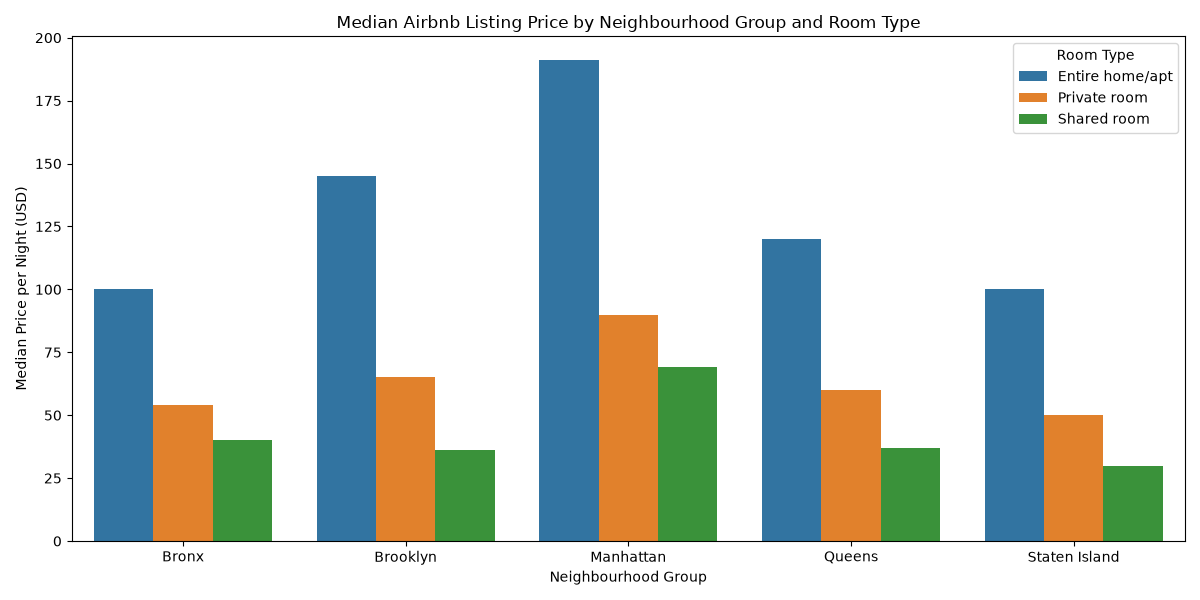
\includegraphics[width=\textwidth]
        {../figures/figure1_median_price.png}
    \caption{Median Airbnb listing price by neighbourhood group and room type.}
    \label{fig:median-price}
\end{figure}

\subsection{Price Distributions}

Figure~\ref{fig:price-distribution} shows that the distributions differ clearly
by room type. Entire homes and apartments have both the highest median and the
widest interquartile range. Private and shared rooms are concentrated at lower
prices, although both categories still contain relatively expensive listings.

All three distributions are right-skewed and contain many observations above
their upper box-plot whiskers. These observations are statistical outliers
under the box-plot convention but are not necessarily erroneous records. The
figure therefore supports retaining the observations while using median values
to describe typical prices.

\begin{figure}[H]
    \centering
    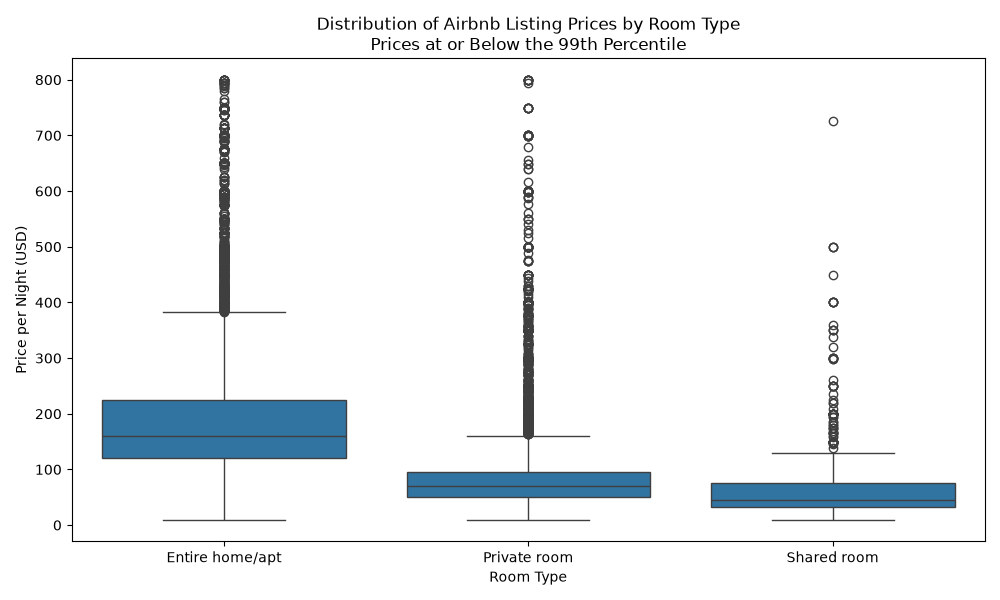
\includegraphics[width=0.9\textwidth]
        {../figures/figure2_price_distribution.png}
    \caption{Distribution of listing prices by room type for prices at or below
    the 99th percentile.}
    \label{fig:price-distribution}
\end{figure}

\subsection{Annual Availability}

Figure~\ref{fig:availability} shows substantial variation in median annual
availability. Staten Island has the highest typical availability for private
rooms, at approximately 280 days, and for entire homes and apartments, at
approximately 175 days. Manhattan and Brooklyn have much lower median
availability for these categories, generally below 50 days.

Shared rooms show a different pattern. Their median availability is relatively
high in Brooklyn and Queens but low in Staten Island. The results indicate that
availability patterns depend on the combination of neighbourhood group and
room type.

A total of 17,530 listings, or 35.86\% of the cleaned dataset, have zero
recorded availability. The proportion is highest in Brooklyn at 39.02\%,
followed by Manhattan at 37.40\%. Staten Island has the lowest proportion at
11.26\%.

\begin{figure}[H]
    \centering
    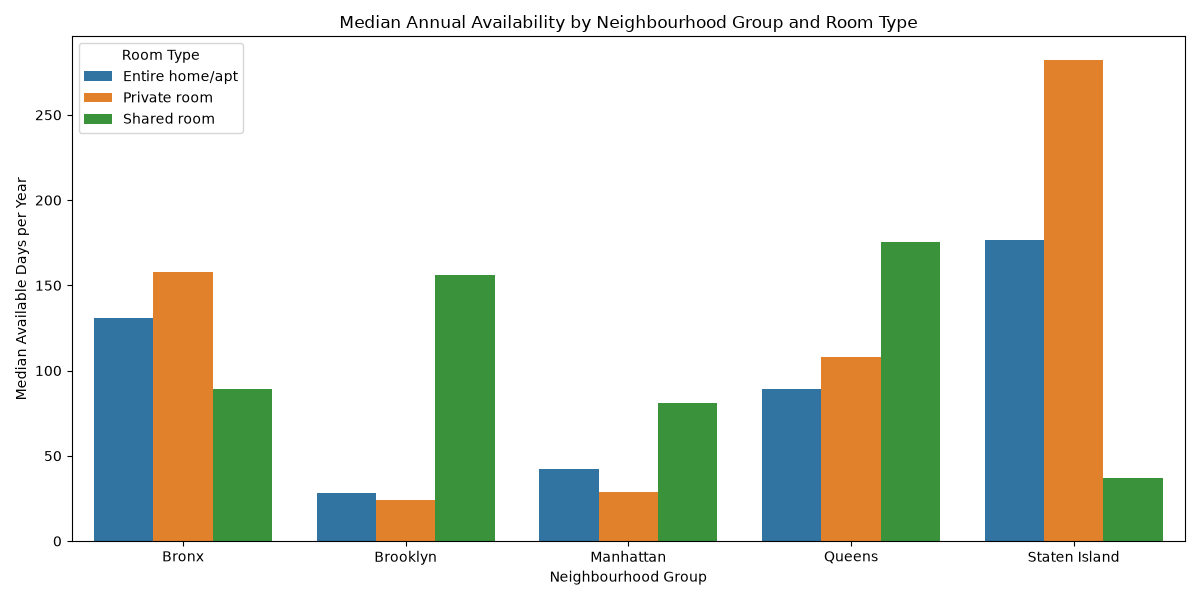
\includegraphics[width=\textwidth]
        {../figures/figure3_availability.png}
    \caption{Median annual availability by neighbourhood group and room type.}
    \label{fig:availability}
\end{figure}

\subsection{Numerical Correlations}

Most numerical variables have only weak linear relationships, as shown in
Figure~\ref{fig:correlation}. The strongest correlation is between
\texttt{number\_of\_reviews} and \texttt{reviews\_per\_month}, with a
coefficient of 0.59. This moderate positive association is expected because
both variables measure review activity.

A weaker but more substantively interesting relationship occurs between
\texttt{calculated\_host\_listings\_count} and
\texttt{availability\_365}, with a coefficient of 0.23. Listings associated
with hosts managing more properties tend to have slightly greater recorded
availability, but this relationship is weak and cannot establish causation.

Price has very weak correlations with all included numerical variables. Its
largest numerical correlation is only 0.08, with annual availability. The
grouped results therefore suggest that neighbourhood group and room type are
more informative for describing price differences than the numerical variables
included in the correlation analysis.

\begin{figure}[H]
    \centering
    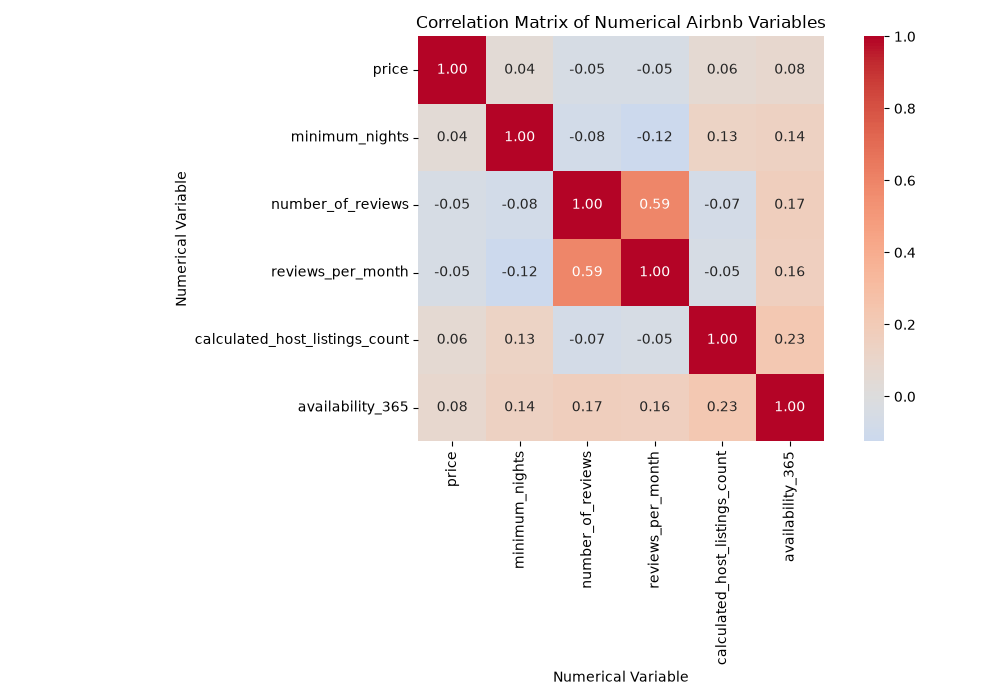
\includegraphics[width=0.82\textwidth]
        {../figures/figure4_correlation.png}
    \caption{Pearson correlation matrix for selected numerical variables.}
    \label{fig:correlation}
\end{figure}

\section{Responsible Practice: Bias and Data Quality}

The findings are descriptive and should not be interpreted as causal. The
dataset does not include several characteristics that may influence price,
including property size, bedroom count, amenities, property condition,
proximity to attractions, and public-transport access. Price differences
associated with neighbourhood group or room type may therefore partly reflect
unobserved variables.

The neighbourhood groups are also unevenly represented. Manhattan and Brooklyn
together account for more than 85\% of the cleaned observations, while Staten
Island accounts for less than 1\%. Aggregate findings are consequently
dominated by Manhattan and Brooklyn, and conclusions about smaller groups are
based on much smaller samples. The shared-room category is also limited,
particularly in Staten Island, where only nine shared-room listings are
present.

The \texttt{availability\_365} variable is ambiguous. Low availability could
indicate frequent bookings, but it could also result from host-blocked dates,
seasonal operation, or an inactive listing. High availability could indicate
lower demand, greater supply, or a newly created listing. Availability was
therefore not treated as a direct measure of occupancy or demand.

Open datasets should not automatically be assumed to represent verified ground
truth. Alsudais documents systemic collection errors and reproducibility
problems across releases of the Inside Airbnb dataset
\parencite{alsudais2020}. Although the present dataset was obtained
from Kaggle rather than directly from an Inside Airbnb release, the same general
caution applies to third-party platform data. The report therefore identifies
the exact dataset source, retains the original CSV, documents all cleaning
rules, and limits its conclusions to the supplied snapshot.

Future work could reduce these risks by validating selected listings against
another source, documenting a precise download date or version, examining
individual neighbourhood sample sizes, and repeating the analysis with data
from additional collection periods.
\section{Reproducibility}

The repository contains the original dataset, the complete Jupyter Notebook,
the generated figures, this report, a \texttt{requirements.txt} file, and a
short README with execution instructions. A reviewer can create a virtual
environment, install the pinned dependencies with

\begin{verbatim}
pip install -r requirements.txt
\end{verbatim}

and run all cells in \texttt{data\_workflow.ipynb} from top to bottom.

The notebook uses relative file paths, reusable functions, explicit cleaning
rules, and intermediate validation checks. The unmodified data are stored in
\texttt{df}, while the cleaned data are stored separately in
\texttt{df\_clean}. This separation preserves the original input and makes the
transformations easier to inspect.

Git was used to record progress through multiple commits. Development work was
performed on an additional branch before being integrated with the main branch.
The commit history documents the progression from repository setup through
data ingestion, cleaning, exploratory analysis, visualization, interpretation,
and reporting.

These practices support computational reproducibility by preserving the code,
data, software dependencies, and development history needed to repeat the
analysis \parencite{danchev2022}.

\clearpage
\printbibliography[title={References},heading=bibintoc]

\appendix
\chapter{Supplementary Material}

Place questionnaires, extended tables, source code excerpts, or other supporting
material here when appropriate.


\end{document}
